\subsection{Equivalence Model}


\begin{frame}
\frametitle{Regex Equivalence Classes}
\begin{figure}[h]
  \centering
  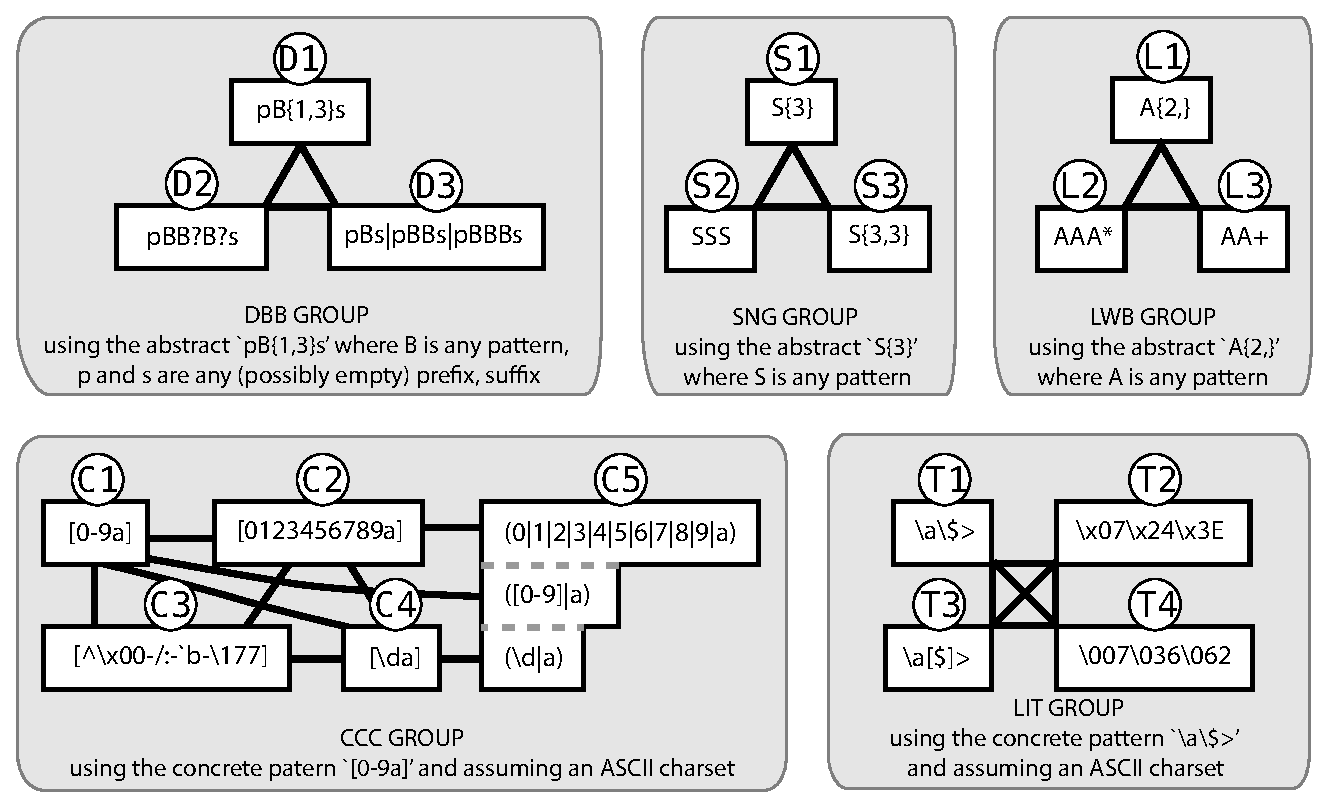
\includegraphics[scale=0.45]{nontex/illustrations/refactoringTree.eps}
  \label{fig:refactoringTree}
\end{figure}
\end{frame}
\note[itemize]{
    \item pt 1
    \item pt 2
}

%------------------------------------------------


\begin{frame}[fragile]
\frametitle{Example Equivalences}
\begin{description}
\item [LIT]: \cverb!x! $\equiv$ \cverb!y!
\item [DBB]: another one
\item [CCC]: a = b
\item [LWB]: another one
\item [SNG]: a = b
\end{description}
\end{frame}
\note[itemize]{
    \item pt 1
    \item pt 2
}

%------------------------------------------------
% \begin{columns}[c] % The "c" option specifies centered vertical alignment while the "t" option is used for top vertical alignment
% \column{.45\textwidth} % Left column and width
% \textbf{Heading}
% \begin{enumerate}
% \item anchored
% \item anchored
% \item anchored
% \end{enumerate}
% \column{.5\textwidth} % Right column and width
% \begin{enumerate}
% \setcounter{enumi}{3}
% \item anchored
% \item anchored
% \item anchored
% \end{enumerate}
% \end{columns}
